\chapter{Save Page}

The Save Page is used to save track data from the Machinedrum or AnalogFour to a specific slots in the current row of the Grid.

When a MD's track is saved to a slot, the track's Machine settings and the MC's internal sequencer data for the chosen track are stored together.

Similarly, when an A4 track is saved, the Sound Settings for the chosen track together with the internal sequencer data are stored together.

\textbf{To retain the MD's pattern data for the selected track(s), you must use the sequencer Merge functionality described below.}

Master Effects settings are also saved with each MD Track.
%\fbox{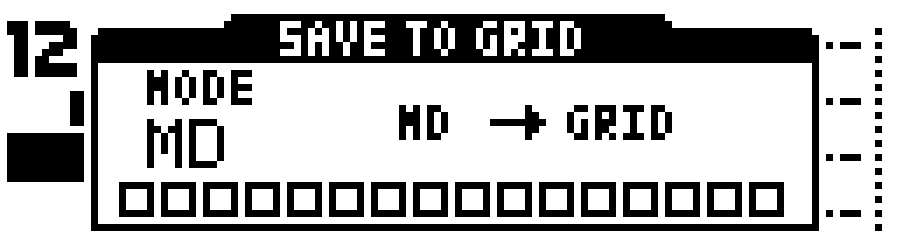
\includegraphics[scale=.40]{save_page.png}}\\

\screenshot{save_to_grid.png}

\textit{The Save Page is accessible from the GridPage by pressing the  \textbf{[Save]} function button.}

\encodersbuttons{Merge}{--}{--}{--}{cancels the save.}{--}{--}{save all tracks.}

\vspace{-0.5cm}

\section{Merge:}

\vspace{-0.5cm}

\screenshot{save_to_grid_merge.png}

The Merge option specifies whether to merge the MD's pattern data in to the internal sequencer. When the merge option is active, the data flow will be updated on the display.

\textit{Note: The Merge option is only available when the sequencer playback is stopped.}

\section{Saving Individual Tracks}
The Save Page uses the Trigger Interface to specify which tracks are to be saved. Pressing multiple trigger buttons on the MD and then releasing them will cause the selected tracks to be stored in the corresponding slots of the current row.

Similary, notes C -> F allow saving Analog4 tracks 1 to 4.
\section{Store a pattern/row:}
To save an entire pattern/row press \textbf{[Shift2]} from within the Save Page. All A4 sounds or external sequencer data will also be saved.



